\documentclass[aspectratio=169]{ISAE-Beamer}
\usefonttheme[onlymath]{serif}
\usepackage{amsmath,amssymb,amsthm}
\usepackage{bm}
\usepackage{color}
\definecolor{theme}{RGB}{0,73,114}

\usepackage{graphicx}
\usepackage{diffcoeff}
\usepackage{dsfont}
\usepackage{mathrsfs}
\usepackage[most]{tcolorbox}

%\usepackage{multimedia}
\usepackage{media9}
\usepackage[backend=bibtex,doi=false,isbn=false,url=false,eprint=false]{biblatex}

\graphicspath{{../images/}}

\bibliography{../mybibliography}

% Math macros
\DeclareMathOperator*{\grad}{grad}
\DeclareMathOperator*{\Grad}{Grad}
\DeclareMathOperator*{\Div}{Div}
\renewcommand{\div}{\operatorname{div}}
\DeclareMathOperator*{\Hess}{Hess}
\DeclareMathOperator*{\curl}{curl}
\DeclareMathOperator{\Tr}{Tr}
\DeclareMathOperator{\Dom}{Dom}
\DeclareMathOperator*{\esssup}{ess\,sup}

\newcommand{\bbR}{\mathbb{R}}
\newcommand{\bbF}{\mathbb{F}}
\newcommand{\bbA}{\mathbb{A}}
\newcommand{\bbB}{\mathbb{B}}
\newcommand{\bbS}{\mathbb{S}}

\newcommand*{\norm}[1]{\ensuremath{\left\|#1\right\|}}
\newcommand{\where}{\qquad \text{where} \qquad}
\newcommand{\inner}[3][]{\ensuremath{\left\langle #2, \, #3 \right\rangle_{#1}}}
\newcommand{\bilprod}[2]{\left\langle \left\langle \, #1, #2 \, \right\rangle \right\rangle}
\newcommand{\pder}[2]{\ensuremath{\partial_{#2} #1}}
\newcommand{\dder}[2]{\ensuremath{\delta_{#2} #1}}
\newcommand{\secref}[1]{\S\ref{#1}}
\newcommand{\energy}[1]{\frac{1}{2} \int_{\Omega} \left\{ #1 \right\} \d\Omega}
\newcommand{\crmat}[1]{\ensuremath{\left[#1\right]_\times}}
\newcommand{\fenics}{\textsc{FEniCS}\xspace}
\newcommand{\firedrake}{\textsc{Firedrake}\xspace}

\DeclareMathOperator*{\argmax}{arg\,max}
\DeclareMathOperator*{\argmin}{arg\,min}

\newtheorem{proposition}{Proposition}
\newtheorem{remark}{Remark}

\def\onedot{$\mathsurround0pt\ldotp$}
\def\cddot{% two dots stacked vertically
	\mathbin{\vcenter{\baselineskip.67ex
			\hbox{\onedot}\hbox{\onedot}}%
}}

\renewcommand\bibfont{\scriptsize}


\makeatletter \renewcommand\d[1]{\ensuremath{%
		\;\mathrm{d}#1\@ifnextchar\d{\!}{}}}
\makeatother

\title[PHD Defense]{A port-Hamiltonian formulation of flexible structures \\
Modelling and structure preserving finite element discretization}

%\institute[ISAE]
%{\inst{1}ISAE-SUPAERO, Toulouse}

\author[Andrea Brugnoli]{Andrea Brugnoli\\
	{\and} \\
	{\textit{Supervisors}} \\
	{Daniel Alazard} \\ {Val\'erie Pommier-Budinger}}

\date[Toulouse, 9/11/20]{November, the 9th, 2020}

%\thanks{}

\begin{document}

\maketitle

\begin{frame}{Outline}

\tableofcontents

\end{frame}

\section{Introduction}

\begin{frame}{Twenty years of distributed port-Hamiltonian systems}

\begin{block}{Distributed port-Hamiltonian systems \only<2>{(Linear case)}}
\begin{equation*}
\begin{aligned}
\partial_t {\bm{\alpha}} &= \mathcal{J} \, \bm{e}, \\
\bm{e} &:= \only<1>{\delta_{\bm{\alpha}}{H}} \only<2>{\mathcal{Q}\bm{\alpha}}, \\
\bm{u}_\partial &= \mathcal{B}_\partial  \, \bm{e}, \\
\bm{y}_\partial &= \mathcal{C}_\partial \, \bm{e}, 
\end{aligned} \qquad
\begin{aligned}
\bm{\alpha} &\quad\text{Energy variables},\\
\bm{e} &\quad\text{Co-energy variables},\\
\bm{u}_\partial &\quad\text{Control input}, \\
\bm{y}_\partial &\quad\text{Control output}. 
\end{aligned} \qquad
\begin{aligned}
\mathcal{J} &\quad\text{Interconnection operator},\\
\only<2>{\mathcal{Q} &\quad\text{Positive operator},}\\
\mathcal{B}_\partial &\quad\text{Input operator}, \\
\mathcal{C}_\partial &\quad\text{Output operator}. \\
\end{aligned}
\end{equation*}
\end{block}
	
They have been used for simulating and controlling a variety of applications:
\begin{itemize}
	\item {flexible thin beams;}
	\item {acoustic waves;}
	\item {stirred tank reactors;}
	\item {plasma in tomahawks;}
	\item {fluid-structure interactions.}
\end{itemize}

\end{frame}

\begin{frame}{Motivation \& Research Objectives}

\begin{alertblock}{A missing piece in the port-Hamiltonian literature}
Despite all the preexisting literature, models arising from structural mechanics on multidimensional geometrical domains have rarely been considered\footfullcite{macchelli2005mindlin}. 
\end{alertblock}

\begin{block}{Purpose of this work}
This thesis tries to establish a clear connection between linear structural mechanics models
and port-Hamiltonian systems, both for the modelling and discretization tasks.
\end{block}

\begin{exampleblock}{Methodologies}
The numerical implementation relies on efficient and well-established libraries, so to avoid constructing everything from scratch.
\end{exampleblock}

\end{frame}

\section{Port-Hamiltonian formulation of Elasticity and Thermoelasticity}

\subsection{Linear elasticity}

\begin{frame}{The Linear Elastodynamics problem}
\begin{overlayarea}{\textwidth}{\textheight}
For small deformations, the displacement within a continuum $\bm{u}$ satisfies the PDE
\begin{equation*}
\rho \diffp[2]{\bm{u}}{t} - \Div(\bm{\mathcal{D}} \Grad \bm{u}) =0, \qquad \bm{x} \in \Omega \subset \bbR^d, \; d \in \{2,3\}.
\end{equation*}
\only<1>{
\begin{itemize}
\item $\rho$ mass density;
\item $\bm{\mathcal{D}}(\cdot) = \frac{E}{1 + \nu} \left[(\cdot) + \frac{\nu}{1-2\nu}\Tr(\cdot) \bm{I} \right]$ the stiffness tensor;
\item $\Grad \bm{u} = \frac{1}{2}\left[\nabla\bm{u} + \nabla^\top\bm{u} \right]$ the symmetric gradient;
\item $\bm{\Sigma} = \bm{\mathcal{D}} \bm{\varepsilon}, \; \bm{\varepsilon} = \Grad \bm{u}$ the stress and strain tensors;
\item $\Div \bm{\Sigma} = \left(\sum_{i=1}^d \diffp{\Sigma_{ij}}{x_i}\right)_{1\le j\le d }$ the tensor divergence.
\end{itemize}
}
\only<2>{
\begin{figure}
	\centering
	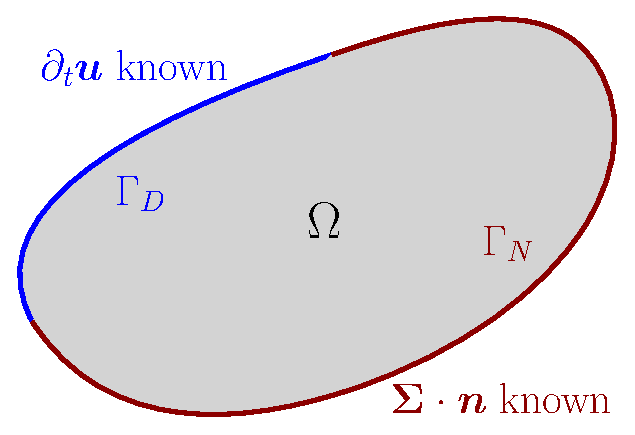
\includegraphics[height=0.5\textheight]{part_2/bc_elas2D.eps}
	\caption{A 2D continuum with Neumann and Dirichlet boundary conditions}
\end{figure}
}
\end{overlayarea}
\end{frame}

\begin{frame}{Energies and co-energies}
\begin{overlayarea}{\textwidth}{\textheight}
	To derive a pH formulation, the total energy is needed
	\begin{equation*}
	H = \energy{\rho \norm{\partial_t \bm{u}}^2 + \bm{\Sigma} \cddot \bm{\varepsilon}}, \qquad \bm{A} \cddot \bm{B} \quad \text{Tensor contraction}.
	\end{equation*}
	\onslide<2->{
	Consider the energy variables
	\[\bm{\alpha}_v = \rho \partial_t \bm{u}, \qquad \bm{A}_{\varepsilon} = \bm{\varepsilon}. \]
	The Hamiltonian is a quadratic functional in this variables
	\begin{equation*}
	H(\bm{\alpha}_v, \bm{A}_{\varepsilon}) = \energy{\frac{1}{\rho} \norm{\bm{\alpha}_v}^2 + (\bm{\mathcal{D}} \bm{A}_{\varepsilon}) \cddot  \bm{A}_{\varepsilon}}.
	\end{equation*} 
	}
	\only<3>{The co-energies are consequently obtained
	\begin{equation*}
	\bm{e}_v = \diffd{H}{\bm{\alpha}_v} = \partial_t \bm{u}, \qquad \bm{E}_{\varepsilon} = \diffd{H}{\bm{A}_{\varepsilon}} = \bm{\mathcal{D}} \bm{A}_{\varepsilon} = \bm{\Sigma}.
	\end{equation*}
	}
\end{overlayarea}
\end{frame}

\begin{frame}{Interconnection operator and boundary variables}
\begin{equation*}
\displaystyle
\diffp{}{t}
\begin{pmatrix}
\bm{\alpha}_v \\
\bm{A}_\varepsilon
\end{pmatrix} = \underbrace{
	\begin{bmatrix}
	\bm{0} & \Div \\
	\Grad & \bm{0} \\
	\end{bmatrix}}_{\mathcal{J}}
\begin{pmatrix}
\bm{e}_v \\
\bm{E}_\varepsilon
\end{pmatrix}, \qquad \begin{aligned}
\text{Dynamics,} \\ \text{Compatibility.}
\end{aligned}
\end{equation*}
\begin{theorem}{}
	The formal anti-adjoint of the $\Div$ operator is the symmetric gradient $\Grad$.
\end{theorem}
From the time derivative of the Hamiltonian, the classical boundary conditions are retrieved
\begin{equation*}
\begin{aligned}
\dot{H} &= \int_{\Omega} \left\{\bm{e}_v \cdot \Div \bm{E}_\varepsilon + \bm{E}_\varepsilon \cddot \Grad \bm{e}_v \right\}\d\Omega, \qquad &\text{Stokes theorem},\\
&= \int_{\partial \Omega} \bm{e}_v \cdot (\bm{E}_\varepsilon\bm{n}) \d{S} = \inner[\partial\Omega]{\bm\gamma_{0}\bm{e}_v}{\bm\gamma_{n}\bm{E}_\varepsilon}.
\end{aligned}
\end{equation*}
The boundary variables are therefore the Dirichlet trace of the velocity $\bm\gamma_{0}\bm{e}_v$ and the normal trace of the stress tensor $\bm\gamma_{n}\bm{E}_\varepsilon$.
\end{frame}


\begin{frame}{The port-Hamiltonian formulation}
	Given the fact that mixed boundary conditions are considered, the trace operators are restricted to the boundary partitions:
	\begin{itemize} 
		\item $\bm\gamma_{0}^{\Gamma_*}$ denotes the Dirichlet trace over the set $\Gamma_*$, $\bm\gamma_{0}^{\Gamma_*} \bm{e}_v = \bm{e}_v\vert_{\Gamma_*}$;
		\item $\bm\gamma_{n}^{\Gamma_*}$ denotes the normal trace over the set $\Gamma_*$, $\bm{\gamma_{n}}^{\Gamma_*}\bm{E}_\varepsilon = \bm{E}_\varepsilon \bm{n}\vert_{\Gamma_*}$.
	\end{itemize}

	\begin{block}{PH linear elasticity}
	\begin{equation*}
	\begin{aligned}
	\displaystyle
	\diffp{}{t}
	\begin{pmatrix}
	\bm{\alpha}_v \\
	\bm{A}_\varepsilon
	\end{pmatrix} &= \underbrace{
		\begin{bmatrix}
		\bm{0} & \Div \\
		\Grad & \bm{0} \\
		\end{bmatrix}}_{\mathcal{J}}
	\begin{pmatrix}
	\bm{e}_v \\
	\bm{E}_\varepsilon
	\end{pmatrix}, \\
	\bm{u}_\partial &= \underbrace{
		\begin{bmatrix}
		\textcolor{blue}{\bm\gamma_{0}^{\Gamma_D}} & \bm{0} \\
		\bm{0} & \textcolor{red}{\bm\gamma_n^{\Gamma_N}} \\
		\end{bmatrix}}_{\mathcal{B}_\partial} \begin{pmatrix}
	\bm{e}_v \\
	\bm{E}_\varepsilon
	\end{pmatrix}, \vspace{3pt}\qquad
	\end{aligned}
	\begin{aligned}
	\begin{pmatrix}
	\bm{e}_v \\
	\bm{E}_\varepsilon
	\end{pmatrix} &= 
	\underbrace{
		\begin{bmatrix}
		\frac{1}{\rho} & \bm{0} \\
		\bm{0} & \bm{\mathcal{D}} \\
		\end{bmatrix}}_{\mathcal{Q}}
	\begin{pmatrix}
	\bm{\alpha}_v \\
	\bm{A}_\varepsilon
	\end{pmatrix}, \\
	\bm{y}_\partial &= \underbrace{
		\begin{bmatrix}
		\bm{0} & \textcolor{blue}{\bm\gamma_{n}^{\Gamma_D}} \\
		\textcolor{red}{\bm\gamma_0^{\Gamma_N}} & \bm{0} \\
		\end{bmatrix}}_{\mathcal{C}_\partial}
	\begin{pmatrix}
	\bm{e}_v \\
	\bm{E}_\varepsilon
	\end{pmatrix}.
	\end{aligned}
	\end{equation*}
	\end{block}
\end{frame}

\begin{frame}{Main steps for the derivation}
The derivation of the Hamiltonian system relies on few simple steps  
\begin{enumerate}
\item Starting from the total energy, the energy variables are selected to make the Hamiltonian quadratic: the new variables are the linear momentum and the strain tensor;
\item The resulting dynamics is regulated by a formally skew-adjoint operator $\mathcal{J}$;
\item The boundary variables are found thanks to the Stokes theorem
\[
\int_{\Omega} \left\{\bm{e}_v \cdot \Div \bm{E}_\varepsilon + \bm{E}_\varepsilon \cddot \Grad \bm{e}_v \right\}\d\Omega = \inner[\partial\Omega]{\bm{e}_v}{\bm{E}_\varepsilon\bm{n}}.
\]
\end{enumerate}

The construction is exactly the same for plate models, as they represent particular cases of this problem.
\end{frame}

\subsection{Plate models: Kirchhoff and Mindlin plates}

\begin{frame}{The Mindlin plate classical model}
Model describing the bending deflection of thick plates
\begin{equation*}
\begin{aligned}
\rho h \diffp[2]{w}{t} &= \div \bm{q}, \qquad (x,y) \in \Omega \subset \bbR^2, \\
\frac{\rho h^3}{12} \diffp[2]{\bm{\theta}}{t} &=\Div \bm{M} + \bm{q},
\end{aligned}
\end{equation*}

\begin{itemize}
	\item $h$ plate thickness;
	\item $\bm{M}= \bm{\mathcal{D}}_b\,\bm{\kappa}$ the momenta tensor;
	\item  $\bm{\kappa} = \Grad{\bm{\theta}}$ the curvature tensor;
	\item $\bm{\mathcal{D}}_{b} = \frac{E h^3}{12(1-\nu^2)} \left[ (1-\nu) (\cdot) + \nu \Tr(\cdot) \bm{I}_{2\times 2} \right]$ the bending stiffness tensor;
	\item $\bm{q}= K_{\text{sh}} Gh\,\bm{\gamma}$ the shear stress ($G$ is the shear modulus and $K_{\text{sh}}$ the shear correction factor);
	\item $\bm{\gamma} = \grad w - \bm{\theta}$ the shear strain.
\end{itemize}

\end{frame}

\begin{frame}{Mindlin plate boundary conditions}
\begin{overlayarea}{\textwidth}{\textheight}
\begin{table}
	\centering
	\begin{tabular}{cc|cc}
		\hline 
		\multicolumn{2}{c}{Dirichlet conditions}&  \multicolumn{2}{c}{Neumann conditions} \\ 
		\hline 
		Vertical velocity  & $w_t = \partial_t {w}$ & Shear force  & $q_n = \bm{q} \cdot \bm{n}$ \\ 
		Flexural rotation  & $\omega_n = \partial_t {\bm{\theta}} \cdot \bm{n}$ & Flexural momentum & $M_{nn} = \bm{n}^\top\bm{M}\bm{n}$ \\  
		Torsional rotation & $\omega_s = \partial_t {\bm{\theta}} \cdot \bm{s}$ & Torsional momentum  & $ M_{ns} = \bm{s}^\top\bm{M}\bm{n}$  \\ 
		\hline 
	\end{tabular}
\end{table}
\only<1>{
\begin{figure}[t]
\centering
\includegraphics[width=0.6\textwidth]{part_2/cauchy_law.eps}
\end{figure}
}
\only<2>{
\begin{figure}[tb]
	\centering
	\includegraphics[width=0.6\textwidth]{part_2/min_plate_bcs.eps}
	\caption{Boundary conditions for the Mindlin plate.}
\end{figure}
}
\end{overlayarea}	

\end{frame}

\begin{frame}{Energies and co-energies for the Mindlin plate}
\begin{overlayarea}{\textwidth}{\textheight}
\begin{block}{Total energy}
	\begin{equation*}
	H = \frac{1}{2} \int_{\Omega}  \left\{ \rho h \left(\diffp{w}{t} \right)^2 + \frac{\rho h^3}{12} \norm{\diffp{\bm{\theta}}{t}}^2 +   \bm{M} \cddot \bm{\kappa} + \bm{q} \cdot \bm{\gamma}  \right\}  \d\Omega, 
	\end{equation*}
\end{block}

\only<1>{
\begin{block}{Energy variables}
	\begin{equation*}
	\begin{aligned}
	\alpha_w &= \rho h \diffp{w}{t}, \quad &\text{Linear momentum,} \\
	\bm{A}_{\kappa} &= \bm{\kappa}, \quad &\text{Curvature tensor,} \\
	\end{aligned} \qquad
	\begin{aligned}
	\bm\alpha_{\theta} &=  \frac{\rho h^3}{12} \diffp{\bm{\theta}}{t}, \quad &\text{Angular momentum,}\\
	\bm\alpha_{\gamma} &= \bm{\gamma}. \quad &\text{Shear deformation.}\\
	\end{aligned}
	\end{equation*}
\end{block}	
}

\only<2>{
\begin{block}{Co-energy variables}
	\begin{equation*}
	\begin{aligned}
	e_w &:= \diffd{H}{\alpha_w} = \diffp{w}{t},  \quad &\text{Linear velocity,} \\
	\bm{E}_{\kappa} &:= \diffd{H}{\bm{A}_{\kappa}} = \bm{M}, \quad &\text{Momenta tensor,}\\
	\end{aligned} \qquad
	\begin{aligned}
	\bm{e}_{\theta} &:= \diffd{H}{\bm\alpha_{\theta}} = \diffp{\bm{\theta}}{t}, \quad &\text{Angular velocity,}  \\
	\bm{e}_{\gamma} &:= \diffd{H}{\bm\alpha_{\gamma}} = \bm{q} \quad &\text{Shear stress.} \\
	\end{aligned}
	\end{equation*}
\end{block}	
}

\end{overlayarea}	
\end{frame}

\begin{frame}{Interconnection operator and boundary variables}
\begin{equation*}\label{eq:pHdyn_Min}
\diffp{}{t}
\begin{pmatrix}
\alpha_w \\
\bm\alpha_\theta \\
\bm{A}_\kappa \\
\bm\alpha_{\gamma} \\
\end{pmatrix} = 
\underbrace{\begin{bmatrix}
0  & 0  & 0  & \div \\
\bm{0} & \bm{0} &  \Div & \bm{I}_{2 \times 2}\\
\bm{0}  & \Grad  & \bm{0}  & \bm{0}\\
\grad & -\bm{I}_{2 \times 2} &  \bm{0} & \bm{0} \\
\end{bmatrix}}_{\mathcal{J}}
\begin{pmatrix}
e_w \\
\bm{e}_{\theta} \\
\bm{E}_{\kappa} \\
\bm{e}_{\gamma} \\
\end{pmatrix}.
\end{equation*}
Again the interconnection operator is formally skew-adjoint. The classical boundary condition are again retrieved from the Hamiltonian
\begin{equation*}
\begin{aligned}
\dot{H}&= \int_{\Omega} \left\{ \div(\bm{e}_{\gamma}) e_w  + \Div(\bm{E}_{\kappa}) \cdot \bm{e}_\theta + \; \Grad(\bm{e}_{\theta}) \cddot \bm{E}_{\kappa}  + \grad (e_w) \cdot \bm{e}_{\gamma} \right\} \d\Omega, \\
&= \inner[\partial\Omega]{\gamma_{0} e_w}{\gamma_{n} \bm{e}_\gamma} + \inner[\partial\Omega]{\gamma_{n}\bm{e}_\theta}{\gamma_{nn}\bm{E}_\kappa} + \inner[\partial\Omega]{\gamma_{s}\bm{e}_\theta}{\gamma_{ns}\bm{E}_\kappa},  \\
\end{aligned}
\end{equation*}
\begin{itemize}
\item $\gamma_{nn}\bm{E}_\kappa = \bm{n}^\top \bm{E}_\kappa \bm{n}\vert_{\partial\Omega}$ denotes the normal-normal trace  of tensor-valued functions;
\item $\gamma_{ns}\bm{E}_\kappa = \bm{s}^\top \bm{E}_\kappa \bm{n}\vert_{\partial\Omega}$ denotes the normal-tangential trace of tensor-valued functions.
\end{itemize}
\end{frame}

\begin{frame}{Mindlin plate as a port-Hamiltonian system}
	\begin{block}{PH Mindlin plate}
		\small
		\setlength{\abovedisplayskip}{1pt}
		\setlength{\belowdisplayskip}{1pt}
		\begin{equation*}
		\begin{aligned}
		\displaystyle
		\diffp{}{t}
		\begin{pmatrix}
		\alpha_w \\
		\bm\alpha_\theta \\
		\bm{A}_\kappa \\
		\bm\alpha_{\gamma} \\
		\end{pmatrix} &= 
		\underbrace{\begin{bmatrix}
			0  & 0  & 0  & \div \\
			\bm{0} & \bm{0} &  \Div & \bm{I}_{2 \times 2}\\
			\bm{0}  & \Grad  & \bm{0}  & \bm{0}\\
			\grad & -\bm{I}_{2 \times 2} &  \bm{0} & \bm{0} \\
			\end{bmatrix}}_{\mathcal{J}}
		\begin{pmatrix}
		e_w \\
		\bm{e}_{\theta} \\
		\bm{E}_{\kappa} \\
		\bm{e}_{\gamma} \\
		\end{pmatrix}, \vspace{3pt}\\
		\bm{u}_\partial &= \underbrace{
			\begin{bmatrix}
			\textcolor{blue}{\gamma_{0}^{\Gamma_C}} & {0} & {0} & {0} \\
			{0} & \textcolor{blue}{\gamma_n^{\Gamma_C}} &  {0} & {0} \\
			{0} & \textcolor{blue}{\gamma_s^{\Gamma_C}} &  {0} & {0} \\
			\textcolor{red}{\gamma_{0}^{\Gamma_S}} & {0} & {0} & {0} \\
			{0} & \textcolor{red}{\gamma_s^{\Gamma_S}} & {0} & {0} \\
			{0} &  {0} & \textcolor{red}{\gamma_{nn}^{\Gamma_S}} & {0} \\
			{0} &  {0} & \textcolor{orange}{\gamma_{nn}^{\Gamma_F}} & {0} \\
			{0} &  {0} & \textcolor{orange}{\gamma_{ns}^{\Gamma_F}} & {0} \\
			{0} &  {0} & {0} & \textcolor{orange}{\gamma_{n}^{\Gamma_F}} \\
			\end{bmatrix}}_{\mathcal{B}_\partial} \begin{pmatrix}
		e_w \\
		\bm{e}_{\theta} \\
		\bm{E}_{\kappa} \\
		\bm{e}_{\gamma} \\
		\end{pmatrix}, 
		\end{aligned} \quad
		\begin{aligned}
		\begin{pmatrix}
		e_w \\
		\bm{e}_{\theta} \\
		\bm{E}_{\kappa} \\
		\bm{e}_{\gamma} \\
		\end{pmatrix} &= 
		\underbrace{\begin{bmatrix}
			\frac{1}{\rho h}  & 0 & 0  & 0 \\
			\bm{0} & \frac{12}{\rho h^3} &  \bm{0} & \bm{0}\\
			\bm{0} & \bm{0} & \bm{\mathcal{D}}_b  & \bm{0}\\
			\bm{0} & \bm{0} &  \bm{0} & K_{\text{sh}} G h \\
			\end{bmatrix}}_{\mathcal{Q}}
		\begin{pmatrix}
		\alpha_w \\
		\bm\alpha_\theta \\
		\bm{A}_\kappa \\
		\bm\alpha_{\gamma} \\
		\end{pmatrix}, \\
		\bm{y}_\partial &= \underbrace{
			\begin{bmatrix}
			{0} & {0} & {0} & \textcolor{blue}{\gamma_{n}^{\Gamma_C}} \\
			{0} & {0} & \textcolor{blue}{\gamma_{nn}^{\Gamma_C}} & {0} \\
			{0} & {0} & \textcolor{blue}{\gamma_{ns}^{\Gamma_C}} & {0} \\
			{0} & {0} & {0} & \textcolor{red}{\gamma_{n}^{\Gamma_S}} \\
			{0} & {0} & \textcolor{red}{\gamma_{ns}^{\Gamma_S}} & {0} \\
			{0} & \textcolor{red}{\gamma_{n}^{\Gamma_S}} & {0} & {0} \\
			{0} & \textcolor{orange}{\gamma_{n}^{\Gamma_F}} & {0} & {0} \\
			{0} & \textcolor{orange}{\gamma_{s}^{\Gamma_F}} & {0} & {0} \\
			\textcolor{orange}{\gamma_{0}^{\Gamma_F}} & {0} & {0} & {0} \\
			\end{bmatrix}}_{\mathcal{C}_\partial}
		\begin{pmatrix}
		e_w \\
		\bm{e}_{\theta} \\
		\bm{E}_{\kappa} \\
		\bm{e}_{\gamma} \\
		\end{pmatrix}.
		\end{aligned}
		\end{equation*}
	\end{block}
\end{frame}

\begin{frame}{Kirchhoff plate classical model}
	This model describes the bending deflection of thin plates
	\begin{equation*}
	\rho h \diffp[2]{w}{t} = - \div\Div \bm{M}, \qquad (x,y) \in \Omega \subset \bbR^2.
	\end{equation*}

	As for the Mindlin plate the stress tensor is defined as 
	$$\bm{M} = \bm{\mathcal{D}}_b \bm{\kappa}.$$
	However, the curvature tensor is now given by the Hessian of the displacement field
	$$\bm{\kappa} = \Grad\grad w = \Hess w.$$
\end{frame}

\begin{frame}{Kirchhoff plate boundary conditions}

\begin{table}
	\centering
	\begin{tabular}{cc|cc}
		\hline 
		\multicolumn{2}{c}{Dirichlet conditions}&  \multicolumn{2}{c}{Neumann conditions} \\ 
		\hline 
		Vertical velocity  & $w_t$ & Effective shear force  & $\widetilde{q}_n = -\Div \bm{M} \cdot \bm{n} - \partial_{\bm{s}} (\bm{s}^\top \bm{M} \bm{n})$ \\ 
		Flexural rotation  & $\partial_{\bm{n}} w_t $  & Flexural momentum & $M_{nn} = \bm{n}^\top\bm{M}\bm{n}$ \\  
		\hline 
	\end{tabular}
\end{table}

\begin{figure}[tb]
	\centering
	\includegraphics[width=0.6\textwidth]{part_2/kirchh_plate_bcs.eps}
	\caption{Boundary conditions for the Kirchhoff plate.}
\end{figure}
		
\end{frame}

\begin{frame}{Energies and co-energies for the Kirchhoff plate}
\begin{overlayarea}{\textwidth}{\textheight}
\begin{block}{Total energy}
	\setlength{\abovedisplayskip}{1pt}
	\setlength{\belowdisplayskip}{1pt}
	\begin{equation*}
	H = \frac{1}{2} \int_{\Omega}  \left\{ \rho h \left(\partial_t {w} \right)^2 + \bm{M} \cddot \bm{\kappa}\right\}  \d\Omega, 
	\end{equation*}
\end{block}
	
\begin{block}{Energy variables}
	\begin{equation*}
	\alpha_w = \rho h \partial_t {w}, \quad \text{Linear momentum,} \qquad
	\bm{A}_{\kappa} = \bm{\kappa}, \quad \text{Curvature tensor.} 
	\end{equation*}
\end{block}	

\begin{block}{Co-energy variables}
	\begin{equation*}
	e_w := \diffd{H}{\alpha_w} = \partial_t {w},  \quad \text{Linear velocity,} \qquad
	\bm{E}_{\kappa} := \diffd{H}{\bm{A}_{\kappa}} = \bm{M}, \quad \text{Momenta tensor.}
	\end{equation*}
\end{block}	
	
\end{overlayarea}	
\end{frame}

\begin{frame}{Interconnection operator and boundary variables}
\begin{equation*}
\diffp{}{t}
\begin{pmatrix}
\alpha_w \\
\bm{A}_{\kappa} \\
\end{pmatrix} = 
\underbrace{\begin{bmatrix}
0  &  - \div \circ \Div \\
\Grad \circ \grad & \bm{0} \\
\end{bmatrix}}_{\mathcal{J}}
\begin{pmatrix}
e_w \\
\bm{E}_{\kappa} \\
\end{pmatrix}.
\end{equation*}

\begin{theorem}
The formal anti-adjoint of the $-\div\Div$ operator is the Hessian operator.
\end{theorem}
Assuming a regular boundary $\partial\Omega \in C^1$
\begin{equation*}
\begin{aligned}
\dot{H}&= \int_{\Omega} \left\{ - \div\Div \bm{E}_{\kappa} \, e_w + \Grad\grad e_w \cddot \bm{E}_{\kappa} \right\} \d\Omega, \\
&=\inner[\partial\Omega]{\gamma_{0} e_w}{\gamma_{nn, 1}\bm{E}_\kappa} + \inner[\partial\Omega]{\gamma_{1} e_w}{\gamma_{nn}\bm{E}_\kappa}.  
\end{aligned}
\end{equation*}
\begin{itemize}
	\item $\gamma_{1} e_w = \partial_{\bm{n}} e_w \vert_{\partial\Omega}$ denote the normal derivative trace;
	\item $\gamma_{nn, 1}$ denotes the map $\gamma_{nn, 1}\bm{E}_\kappa = -\bm{n} \cdot \Div \bm{E}_\kappa - \partial_{\bm{s}} (\bm{s}^\top\bm{E}_\kappa\bm{n})\vert_{\partial\Omega}$.
\end{itemize}
\end{frame}

\begin{frame}{The Kirchhoff plate as a pH system}
	\begin{block}{PH Kirchhoff plate}
		\begin{equation*}
		\begin{aligned}
		\displaystyle
		\diffp{}{t}
		\begin{pmatrix}
		\alpha_w \\
		\bm{A}_{\kappa} \\
		\end{pmatrix} &= 
		\underbrace{\begin{bmatrix}
			0  &  - \div \circ \Div \\
			\Grad \circ \grad & \bm{0} \\
			\end{bmatrix}}_{\mathcal{J}}
		\begin{pmatrix}
		e_w \\
		\bm{E}_{\kappa} \\
		\end{pmatrix}, \vspace{3pt}\\
		\bm{u}_\partial &= \underbrace{
			\begin{bmatrix}
			\textcolor{blue}{\gamma_{0}^{\Gamma_C}} & {0}  \\
			\textcolor{blue}{\gamma_1^{\Gamma_C}} &  {0} \\
			\textcolor{red}{\gamma_{0}^{\Gamma_S}} &  {0}  \\
			{0} & \textcolor{red}{\gamma_{nn}^{\Gamma_S}} \\
			{0} & \textcolor{orange}{\gamma_{nn, 1}^{\Gamma_F}}  \\
			{0} & \textcolor{orange}{\gamma_{nn}^{\Gamma_F}}\\
			\end{bmatrix}}_{\mathcal{B}_\partial} \begin{pmatrix}
		e_w \\
		\bm{E}_{\kappa} \\
		\end{pmatrix}, 
		\end{aligned} \qquad
		\begin{aligned}
		\begin{pmatrix}
		e_w \\
		\bm{E}_{\kappa} \\
		\end{pmatrix} &= 
		\underbrace{\begin{bmatrix}
		\frac{1}{\rho h}  &  0 \\
		\bm{0} & \bm{\mathcal{D}}_b \\
		\end{bmatrix}}_{\mathcal{Q}}
		\begin{pmatrix}
		\alpha_w \\
		\bm{A}_{\kappa} \\
		\end{pmatrix}, \\
		\bm{y}_\partial &= \underbrace{
			\begin{bmatrix}
			{0} & \textcolor{blue}{\gamma_{nn, 1}^{\Gamma_C}} \\
			{0} & \textcolor{blue}{\gamma_{nn}^{\Gamma_C}} \\
			{0} & \textcolor{red}{\gamma_{nn, 1}^{\Gamma_S}} \\
			\textcolor{red}{\gamma_{1}^{\Gamma_S}} & {0} \\
			\textcolor{orange}{\gamma_{0}^{\Gamma_F}} & {0} \\
			\textcolor{orange}{\gamma_{1}^{\Gamma_F}} & {0} \\
			\end{bmatrix}}_{\mathcal{C}_\partial}
		\begin{pmatrix}
		e_w \\
		\bm{E}_{\kappa} \\
		\end{pmatrix}.
		\end{aligned}
		\end{equation*}
	\end{block}
\end{frame}

\subsection{Few words on thermoelasticity}

\begin{frame}{The heat equation as a pHDAE}
\begin{overlayarea}{\textwidth}{\textheight}
Consider the heat equation
\begin{equation*}\label{eq:heatEq}
\rho c_\epsilon \partial_t T = k \Delta T + r_Q, \qquad \quad \bm{x} \in \Omega \subset \mathbb{R}^d,
\end{equation*}
\only<1>{
\begin{itemize}
\item $c_\epsilon$ the specific heat density at constant strain;
\item $k$ the thermal diffusivity;
\item $r_Q$ an heat source.
\end{itemize}
}
\only<2>{
Given the Hamiltonian
\begin{equation*}
H_T = \frac{1}{2} \int_\Omega \rho c_\epsilon T_0 \left(\frac{T-T_0}{T_0} \right)^2 \d\Omega,
\end{equation*}
the energy variable and corresponding co-energy are
\begin{equation*}
\alpha_T := \rho c_\epsilon (T-T_0), \qquad e_T := \delta_{\alpha_T} {H_T} ={T-T_0}/{T_0}.
\end{equation*}
Introducing the heat flux $\bm{j}_Q := -k \grad T$ as algebraic variable
\begin{equation*}
\begin{aligned}
\begin{bmatrix}
1 & 0 \\
\bm{0} & \bm{0} \\
\end{bmatrix}
\diffp{}{t}
\begin{pmatrix}
\alpha_T \\
\bm{j}_Q \\
\end{pmatrix} &= 
\begin{bmatrix}
0 & -\div \\
-\grad & -(T_0 k)^{-1} \\
\end{bmatrix}
\begin{pmatrix}
e_T \\
\bm{j}_Q \\
\end{pmatrix} + 
\begin{bmatrix}
1 \\
\bm{0} \\
\end{bmatrix} u_T, \\
y_T &= \begin{bmatrix}
1 & \bm{0} \\
\end{bmatrix} \begin{pmatrix}
e_T \\
\bm{j}_Q \\
\end{pmatrix}.
\end{aligned}
\end{equation*}
}
\end{overlayarea}

\end{frame}

\begin{frame}{Classical thermoelasticity as two interconnected systems}
Consider again the equation of elasticity with a distributed input $\bm{u}_E$ (a distributed force)
\begin{equation*}
\begin{aligned}
\diffp{}{t}
\begin{pmatrix}
\bm{\alpha}_v \\
\bm{A}_{\varepsilon} \\
\end{pmatrix} &= 
\begin{bmatrix}
\bm{0} & \Div \\
\Grad & \bm{0} \\
\end{bmatrix}
\begin{pmatrix}
\bm{e}_v \\
\bm{E}_{\varepsilon} \\
\end{pmatrix} + 
\begin{bmatrix}
\bm{I}_{d\times d} \\
\bm{0} \\
\end{bmatrix}\bm{u}_E, \\
\bm{y}_E &= \begin{bmatrix}
\bm{I}_{d\times d} & \bm{0} \\
\end{bmatrix}
\begin{pmatrix}
\bm{e}_v \\
\bm{E}_{\varepsilon}
\end{pmatrix},
\end{aligned}
\end{equation*}
and the heat equation
\begin{equation*}
\begin{aligned}
\begin{bmatrix}
1 & 0 \\
\bm{0} & \bm{0} \\
\end{bmatrix}
\diffp{}{t}
\begin{pmatrix}
\alpha_T \\
\bm{j}_Q \\
\end{pmatrix} &= 
\begin{bmatrix}
0 & -\div \\
-\grad & -(T_0 k)^{-1} \\
\end{bmatrix}
\begin{pmatrix}
e_T \\
\bm{j}_Q \\
\end{pmatrix} + 
\begin{bmatrix}
1 \\
\bm{0} \\
\end{bmatrix} u_T, \\
y_T &= \begin{bmatrix}
1 & \bm{0} \\
\end{bmatrix} \begin{pmatrix}
e_T \\
\bm{j}_Q \\
\end{pmatrix},
\end{aligned}
\end{equation*} 

 
 
\end{frame}

\begin{frame}{The interconnection}
 Consider the  interconnection
\begin{equation*}
\bm{u}_E = - \Div(\bm{\mathcal{C}}_\beta \, y_T), \qquad
u_T = - \bm{\mathcal{C}}_\beta \cddot\Grad(\bm{y}_E). 
\end{equation*}
The interconnection is power preserving since
\begin{equation*}
\bm{u}_E = \mathcal{A}_\beta(y_T), \qquad u_T = - \mathcal{A}_\beta^*(\bm{y}_E), \where  \mathcal{A}_\beta(\cdot) = - \Div(\bm{\mathcal{C}}_\beta \, \cdot).
\end{equation*}
\begin{block}{PH thermoelasticity}
The coupled thermoelastic problem can now be written as
\begin{equation*}
\begin{bmatrix}
\bm{1} & \bm{0} & \bm{0} & \bm{0}\\
\bm{0} & \bm{1} & \bm{0} & \bm{0}\\
0 & 0 & 1 & 0\\
\bm{0} & \bm{0} & \bm{0} & \bm{0}\\
\end{bmatrix}
\diffp{}{t}
\begin{pmatrix}
\bm{\alpha}_v \\
\bm{A}_\varepsilon \\
{\alpha}_T \\
\bm{j}_Q \\
\end{pmatrix} = 
\begin{bmatrix}
\bm{0} & \Div & \mathcal{A}_\beta & \bm{0}\\
\Grad & \bm{0} & \bm{0} & \bm{0} \\
- \mathcal{A}_\beta^* & 0 & 0 & -\div \\
\bm{0} & \bm{0} & -\grad & - (T_0 k)^{-1} \\
\end{bmatrix}
\begin{pmatrix}
\bm{e}_v \\
\bm{E}_\varepsilon \\
{e}_T \\
\bm{j}_Q \\
\end{pmatrix},
\end{equation*}
with total energy given by $H=H_E + H_T$.
\end{block}

\end{frame}

\section{A structure preserving discretization method}

\begin{frame}{Structure preserving discretization}
	\begin{tcbraster}[raster columns=2, raster equal height]
		\begin{tcolorbox}[width=0.4\textwidth, nobeforeafter, colframe=theme,title=Infinite-dimensional pH system]%%
			PDE with distributed inputs:
			\begin{align*}
			\diffp{\bm{\alpha}}{t}(\bm{x}, t) &= \mathcal{J} \delta_{\bm{\alpha}} H + \mathcal{B} \textcolor{red}{\bm{u}_\Omega(\bm{x}, t)}, \\
			\textcolor{red}{\bm{y}_\Omega(\bm{x}, t)} &= \mathcal{B}^* \delta_{\bm{\alpha}} H.
			\end{align*}
			Boundary conditions: 
			\[\textcolor{blue}{\bm{u}_\partial} = \mathcal{B}_\partial \delta_{\bm{\alpha}} H, \quad \textcolor{blue}{\bm{y}_\partial} = \mathcal{C}_\partial \delta_{\bm{\alpha}} H. \]
			Power balance (Stokes Theorem): 
			\[ \dot{H} = \displaystyle \int_{\partial \Omega} \textcolor{blue}{\bm{u}_\partial} \cdot \textcolor{blue}{\bm{y}_\partial} \d{S} +  \int_{\Omega} \textcolor{red}{\bm{u}_\Omega} \cdot \textcolor{red}{\bm{y}_\Omega} \d{\Omega}.
			\]
		\end{tcolorbox} 
		\begin{tcolorbox}[width=0.4\textwidth, nobeforeafter,  colframe=theme,title=Structure-preserving discretization]%%
			Resulting ODE:
			\begin{align*}
			\dot{\bm{\alpha}}_d &= \mathbf{J} \, {\nabla {H}_d} + \mathbf{B}_\Omega \textcolor{red}{\mathbf{u}_\Omega} + \mathbf{B}_\partial \textcolor{blue}{\mathbf{u}_\partial}, \\
			\textcolor{red}{\mathbf{y}_\Omega} &= \mathbf{B}_\Omega^\top \, {\nabla {H}_d}, \\
			\textcolor{blue}{\mathbf{y}_\partial} &= \mathbf{B}_\partial^\top \,{\nabla {H}_d}.
			\end{align*}
			Discretized Hamiltonian:
			\[
			H_d := H(\bm{\alpha} \equiv \bm{\alpha}_d).
			\]
			Power balance: 
			\[ \dot{H} = \textcolor{blue}{\mathbf{u}_\partial^\top \mathbf{y}_\partial} +  \textcolor{red}{\mathbf{u}_\Omega^\top \mathbf{y}_\Omega}.
			\]
		\end{tcolorbox}
	\end{tcbraster}
\end{frame}

\begin{frame}{The Kirchoff plate as a pH system}
	content...
\end{frame}

\begin{frame}{}
\begin{exampleblock}{Available methods}
	\begin{itemize}
		\item Spectral methods (Moulla 2012):
		\begin{itemize}
			\item[\textcolor{green}{\checkmark}] Rapid spectral convergence;
			\item[\textcolor{red}{$\times$}] Only for 1D problem;
		\end{itemize}
		\item Finite differences (Trenchant 2018);
		\begin{itemize}
			\item[\textcolor{green}{\checkmark}] Valid up to 2D geometries;
			\item[\textcolor{red}{$\times$}] Requires \textit{ad hoc} implementation (staggered grids);
		\end{itemize}
		\item Finite elements based
		\begin{itemize}
			\item Golo 2004, Kotyczka 2018: the implementation requires exterior calculus knowledge and depends on the some parameters that ensure the preservation of power flow;		
			\item \textcolor{blue}{Cardoso-Ribeiro 2018}:
			\begin{itemize}
				\item[\textcolor{green}{\checkmark}] Natural extension of the mixed finite element method to pH systems;
				\item[\textcolor{green}{\checkmark}] Implementable using well-established libraries (Fenics, Firedrake);
			\end{itemize}
		\end{itemize}
	\end{itemize}
\end{exampleblock}
\end{frame}


\begin{frame}{The partitioned finite element method (PFEM)}
General form of a linear pH system in co-energy variables
\begin{equation*}
\mathcal{M} \diffp{e}{t} = \mathcal{J} e, \qquad \mathcal{M} = \mathcal{Q}^{-1}
\end{equation*}

\begin{block}{General procedure for PFEM}
	\setlength{\abovedisplayskip}{1pt}
	\setlength{\belowdisplayskip}{1pt}
	\begin{enumerate}
		\item Put the system into weak form:
		\begin{equation*}
		\left(v, \mathcal{M} \diffp{e}{t} \right)_{\Omega} = \left(v, \mathcal{J} e \right)_{\Omega}.
		\end{equation*}
		\item Apply integration by part on a partition of $\mathcal{J}$:
		\begin{equation*}
		\left(v, \mathcal{J} e \right)_{\Omega} \overbrace{=}^{i.b.p.} j(v, e)_{\Omega} + b(v, u_\partial)_{\partial \Omega},
		\end{equation*}
		so that $j(v, e)_{\Omega}$ is a skew-symmetric bilinear form.
		\item Discretization by Galerkin method (same basis function for test and co-energy variables)
	\end{enumerate}
\end{block}
\end{frame}



\begin{frame}{Results}
\begin{center}
	\onslide*<1>{
		\setlength{\abovedisplayskip}{0pt}
		\setlength{\belowdisplayskip}{0pt}
		Distributed load ($t_{\text{end}} = 10 \, [\mathrm{ms}]$)
		\begin{equation*}
		p = \begin{cases}
		10^5 \left[ y + 10 \left( y - L_y/2 \right)^2 \right] [Pa], \quad &\forall \, t < 2 \, [\mathrm{ms}], \\
		0, \quad &\forall \, t \ge 2 \, [\mathrm{ms}].
		\end{cases}
		\end{equation*}
		\begin{columns}
			\begin{column}{.45\textwidth}
				\includemedia[
				label=vidNoRod,
				addresource=/home/a.brugnoli/Videos_defense/Kirchh_NoRod.mp4,
				activate=pageopen,
				width=6cm, height=5cm,
				flashvars={
					source=/home/a.brugnoli/Videos_defense/Kirchh_NoRod.mp4
					&loop=true
				}
				]{}{VPlayer.swf}
			\end{column}
			\begin{column}{.45\textwidth}
				\includemedia[
				label=vidRod,
				addresource=/home/a.brugnoli/Videos_defense/Kirchh_Rod.mp4,
				activate=pageopen,
				width=6cm, height=5cm,
				flashvars={
					source=/home/a.brugnoli/Videos_defense/Kirchh_Rod.mp4
					&loop=true
				}
				]{}{VPlayer.swf}
			\end{column}
		\end{columns}
	
	\mediabutton[
	mediacommand=vidNoRod:playPause,
	mediacommand=vidRod:playPause
	]{\fbox{Play/Pause}}
				
		%\movie[width=0.8\textwidth, height=0.6\textheight]{Plate and rod}{../Videos/Comparison_RodNoRod.mp4}	
	}
	
	\end{center}
\end{frame}

\section{Stabilization by boundary injection}

\begin{frame}{Boundary stabilization of the Kirchhoff plate}
\only<1>{Consider the problem
	\begin{equation*}\small
	\begin{bmatrix}
	\rho h & 0 \\ 0 & \mathbb{D}^{-1} \\
	\end{bmatrix}
	\diffp{}{t}
	\begin{bmatrix}
	\partial_t w \\ \bm{M} \\
	\end{bmatrix} = 
	\begin{bmatrix}
	0 & -\div\Div \\ \nabla^2 & 0 \\
	\end{bmatrix}
	\begin{bmatrix}
	\partial_t w \\ \bm{M} \\
	\end{bmatrix} \quad (x, y) \in \Omega = [0, 1]\times[0,1]
	\end{equation*}
	subjected to the following boundary conditions
	\begin{align*}
	\begin{aligned}
	\partial_t w|\textcolor{blue}{\Gamma_D} &= 0, \\
	\partial_x \partial_t w|\textcolor{blue}{\Gamma_D} &= 0, \\
	\end{aligned} \qquad \textcolor{blue}{\Gamma_D} &= \left\{x = 0 \right\}\\
	\begin{aligned}
	{M}_{nn}|\textcolor{red}{\Gamma_N} &= u_M, \; \\
	\widetilde{q}|\textcolor{red}{\Gamma_N} &= u_F,\\
	\end{aligned} \qquad \textcolor{red}{\Gamma_N} &= \left\{y = 0 \cup x=1 \cup y=1 \right\}
	\end{align*}
	
	with initial conditions (compatible with the constraints):
	\[
	\partial_t w(x,y,0) = x^2; \qquad \bm{M}(x,y,0) ={0}.
	\]
}
\only<2>{ Obtain a finite-dimensional uncontrolled system
	\begin{equation*}
	\begin{aligned}
	\begin{bmatrix}
	{M} & {0} \\
	{0} & {0} \\
	\end{bmatrix}\frac{d}{d t}
	\begin{pmatrix}
	\bm{e}\\
	\bm{\lambda} \\
	\end{pmatrix}
	&= \begin{bmatrix}
	{J} & {G} \\
	-{G}^T & {0} \\
	\end{bmatrix}
	\begin{pmatrix}
	\bm{e} \\
	\bm{\lambda} \\
	\end{pmatrix} + \begin{bmatrix}
	{B} \\
	0 \\
	\end{bmatrix} \bm{u}, \\
	{y} &= \begin{bmatrix}
	{B}^T & {0} \\
	\end{bmatrix} \begin{pmatrix}
	\bm{e}\\
	\bm{\lambda} \\
	\end{pmatrix},
	\end{aligned} 
	\end{equation*}
	Apply the control law $\bm{u} = -K\bm{y}, \ K>0$
	\begin{equation*}
	\begin{bmatrix}
	M & {0} \\
	{0} & {0} \\
	\end{bmatrix}
	\frac{d}{d t}
	\begin{pmatrix}
	\bm{e}\\
	\bm{\lambda} \\
	\end{pmatrix}
	= \begin{bmatrix}
	{J} - {R} & {G} \\
	-{G}^T & {0} \\
	\end{bmatrix}
	\begin{pmatrix}
	\bm{e}\\
	\bm{\lambda} \\
	\end{pmatrix},
	\end{equation*}
	with ${R} = {B} {K} {B}^T \succeq 0$. \\
	The Hamiltonian $\dot{H} = - \bm{e}^T R \bm{e} \le 0$ is a non increasing function and by La~Salle principle the equilibrium point $\bm{e} = 0$ is asymptotically stable.	
}

\end{frame}
\begin{frame}
\begin{center}
	\only<1>{Control parameter ($t_{\text{end}} = 5 [\mathrm{s}]$)
		\begin{equation*}
		K = 
		\begin{cases}
		0, \quad &\forall t < 1 \, [\mathrm{s}], \\
		100, \quad &\forall t \ge 1 \, [\mathrm{s}].
		\end{cases}
		\end{equation*}
		\vspace{.1cm} \\
		\includemedia[
		label=vidDam,
		addresource=/home/a.brugnoli/Videos_defense/Kirchh_Damped.mp4,
		activate=pageopen,
		width=10cm, height=5cm,
		flashvars={
			source=/home/a.brugnoli/Videos_defense/Kirchh_Damped.mp4
			&loop=true
		}
		]{}{VPlayer.swf}
		
		\mediabutton[
		mediacommand=vidDam:playPause,
		]{\fbox{Play/Pause}}
		
		%\movie[width=0.42\textwidth, height = 0.7 \textheight]{Damped Kirchhoff Plate}{../Videos/Kirchh_Damped_4faster.mp4}			
	}

\end{center}
\end{frame}

\begin{frame}{Conclusion}
The following has been presented:
	\begin{itemize}
	\onslide<2->{\item the Kirchhoff plate model as a port Hamiltonian system;}
	\onslide<3->{\item a structure preserving discretization method capable of dealing with generic bcs;}
	\onslide<4->{\item interconnection with rigid elements (multibody framework);}
		\onslide<5->{\item a simple control application by damping injection;}
	\end{itemize}
	\onslide<6->{Still no rigorous proof of convergence for the finite elements. Existing solutions (only for static problems):}
	\begin{itemize}
		\onslide<7->{\item The Hellan-Herrmann-Johnson  method, but difficulties when dealing with inhomogeneous bcs;}
		\onslide<8->{\item New discretization method capable that handles inhomogeneous bcs.}
	\end{itemize}
\end{frame}


\begin{frame}{}
\centering
\Huge Thanks for your attention \\
\Huge Questions?
\end{frame}


\begin{comment}
\begin{frame}
\begin{tcbraster}[raster columns=2, raster equal height]
\setlength{\abovedisplayskip}{1pt}
\setlength{\belowdisplayskip}{1pt}
\begin{tcolorbox}[width=0.5\textwidth, nobeforeafter, colframe=blue,title=Dirichlet conditions]%%
\begin{equation*}
\begin{aligned}
\text{Vertical velocity}  \quad w_t &:= \partial_t {w}, \\
\text{Flexural rotation} \quad 
\omega_{n} &:= \partial_t {\bm{\theta}} \cdot \bm{n}, \\
\text{Torsional rotation} \quad 
\omega_{s} &:= \partial_t {\bm{\theta}} \cdot \bm{s},	
\end{aligned}
\end{equation*}
\end{tcolorbox} 
\begin{tcolorbox}[width=0.5\textwidth, nobeforeafter,  colframe=red,title=Neumann conditions]%%
\begin{equation*}
\begin{aligned}
\text{Shear force}  \qquad q_{n} &:= \bm{q} \cdot \bm{n},  \\
\text{Flexural momentum} \quad 
M_{nn} &:=  \bm{n}^\top\bm{M}\bm{n},	\\
\text{Torsional momentum} \quad M_{ns} &:= \bm{s}^\top \bm{M}\bm{n},	
\end{aligned}	
\end{equation*}
\end{tcolorbox}
\end{tcbraster}

\begin{equation*}
\begin{aligned}
\text{Dirichlet conditions} \\
\text{Vertical velocity}  \quad w_t &:= \partial_t {w}, \\
\text{Flexural rotation} \quad 
\omega_{n} &:= \partial_t {\bm{\theta}} \cdot \bm{n}, \\
\text{Torsional rotation} \quad 
\omega_{s} &:= \partial_t {\bm{\theta}} \cdot \bm{s},	
\end{aligned} \qquad 
\begin{aligned}
\text{Neumann conditions} \\
\text{Shear force}  \qquad q_{n} &:= \bm{q} \cdot \bm{n},  \\
\text{Flexural momentum} \quad 
M_{nn} &:=  \bm{M} \cddot (\bm{n}\otimes{\bm{n}}),	\\
\text{Torsional momentum} \quad M_{ns} &:= \bm{M} \cddot (\bm{s}\otimes{\bm{n}}),	
\end{aligned}
\end{equation*}
\end{frame}

\end{comment}

\end{document}
